% !TeX program = latexmk
% !TeX spellcheck = pl_PL
% !TeX root = example.tex

\chapter{Implementacja projektu}

Aplikacja \textit{Planning Poker}, to aplikacja webowa oparta na platformie Firebase,
która jest napisana przy użyciu biblioteki ReactJS, z wykorzystaniem
edytora Visual Studio Code.

Aby zachować porządek i możliwość późniejszego rozwoju aplikacji o nowe komponenty,
koniecznym jest stworzenie uporządkowanej struktury plików zawartych w projekcie
(rysunek~\ref{rys:projekt}).

\begin{figure}[h]
	\centering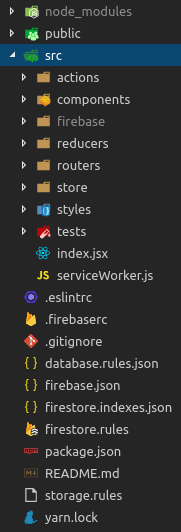
\includegraphics[width=.3\textwidth]{img/projekt.png}
	\caption{Struktura projektu}\label{rys:projekt}% Źródło rysunku i etykieta przez którą odwołujemy się do rysunku.
\end{figure}

Folderem zawierającym wszystkie podfoldery oraz pliki jest folder \texttt{scrumpoker}.
Pliki takie jak \texttt{storage.rules} czy \texttt{.firebaesrc} powstały automatycznie
w procesie konfiguracji usługi Firebase.

Plik \texttt{package.json} zawiera całą konfigurację projektu stworzonego
za pomocą narzędzia \texttt{create-react-app}.

Folder \texttt{node modules} zawiera zależności, niezbędne do uruchomienia aplikacji.

Folder \texttt{src} zawiera cały kod źródłowy aplikacji.
Głównym plikiem projektu jest \texttt{index.jsx}. To w tym pliku renderowana jest cała aplikacja.

Aby uruchomić program,
niezbędny jest też backend w postaci utworzonego i skonfigurowanego projektu Firebase.
Konfiguracje należy umieścić w pliku \texttt{src/firebase/firebase.jsx}
(patrz listing~\ref{listing:firebaseConfig}).

\begin{listing}
\begin{minted}{c}
import * as firebase from 'firebase';

var config = {
    apiKey: "<API_KEY>",
    authDomain: "<PROJECT_ID>.firebaseapp.com",
    databaseURL: "https://<DATABASE_NAME>.firebaseio.com",
    projectId: "<PROJECT_ID>",
    storageBucket: "<BUCKET>.appspot.com",
    messagingSenderId: "<SENDER_ID>",
};

firebase.initializeApp(config);

const database = firebase.firestore();
const settings = { timestampsInSnapshots: true};
database.settings(settings);
export { firebase, database as default };
\end{minted}
\caption{Konfiguracja firebase}\label{listing:firebaseConfig}
\end{listing}

Z wyjątkiem stanu gry, aplikacja wszelkie dane pobiera z serwisu Github poprzez
udostępnione API, wykorzystując do tego biliotekę \texttt{octokit/rest}.

W każdym komponencie, wymagającym danych z tego serwisu,
uruchamiane są metody, które ładują niezbędne dane do stanu komponentu.

Jako że wszelkie gry tworzone w aplikacji dotyczą projektów prowadzonych na Github'ie,
użytkownik, aby skorzystać z aplikacji, musi posiadać konto na Github'ie oraz co najmniej
jeden projekt założony w tej usłudze.
Biorąc pod uwagę, że w trakcie rozgrywki Planning Pokera oceniane są historyjki z backlogu,
użytkownik musi mieć jakieś historyjki przypisane do wybranego projektu w Github.
Aby to zrobić musi utworzyć w projekcie, elementy zwane `issues', które w tym momencie traktowane są jako historyjki.
Co za tym idzie, użytkownik musi się zalogować przez serwis Github, co ilustruje poniższy rysunek~\ref{rys:login}.

\begin{figure}[h]
	\centering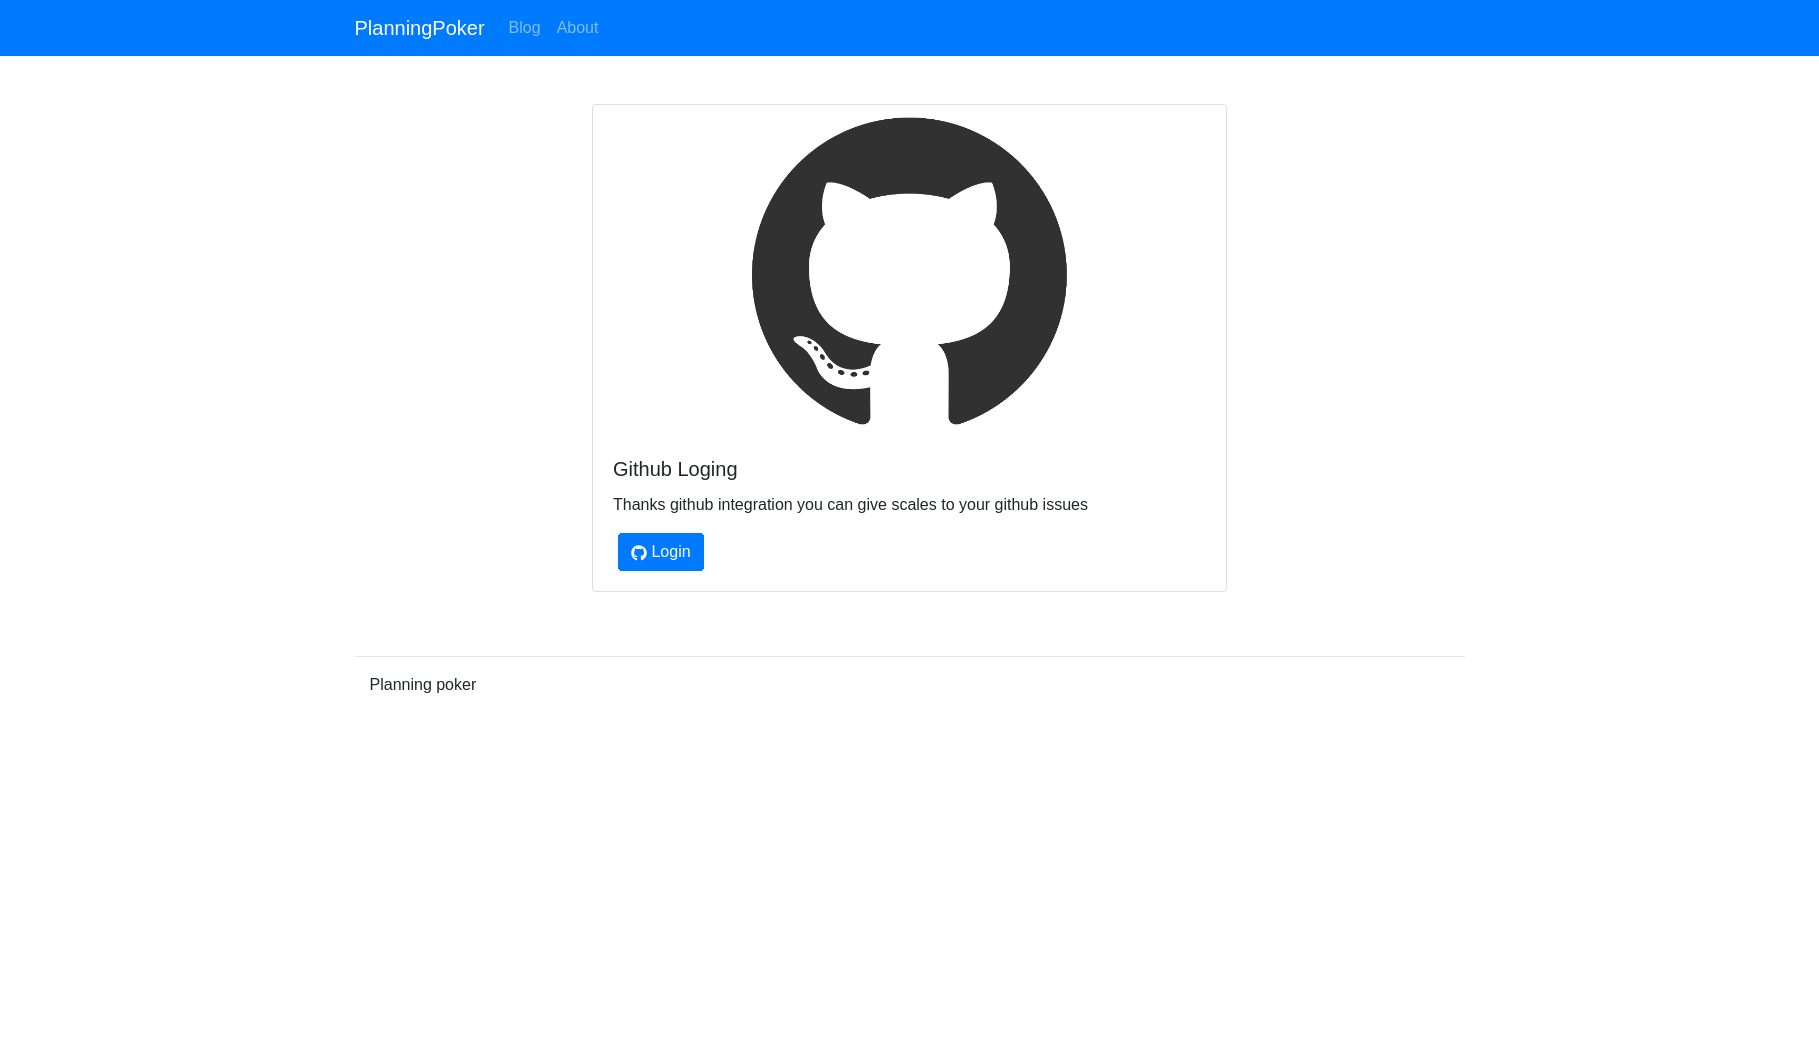
\includegraphics[width=\textwidth]{img/GitLogin.png}
	\caption{Strona logowania}\label{rys:login}% Źródło rysunku i etykieta przez którą odwołujemy się do rysunku.
\end{figure}

\section{Tworzenie gry}

Można założyć, że grupą docelową aplikacji, są użytkownicy Githuba, czyli programiści.
Autor, jako częsty użytkownik tej usługi, odczuł brak aplikacji wspomagającej Planning Poker,
która byłaby z tym narzędziem zintegrowana.

\begin{figure}[h]
	\centering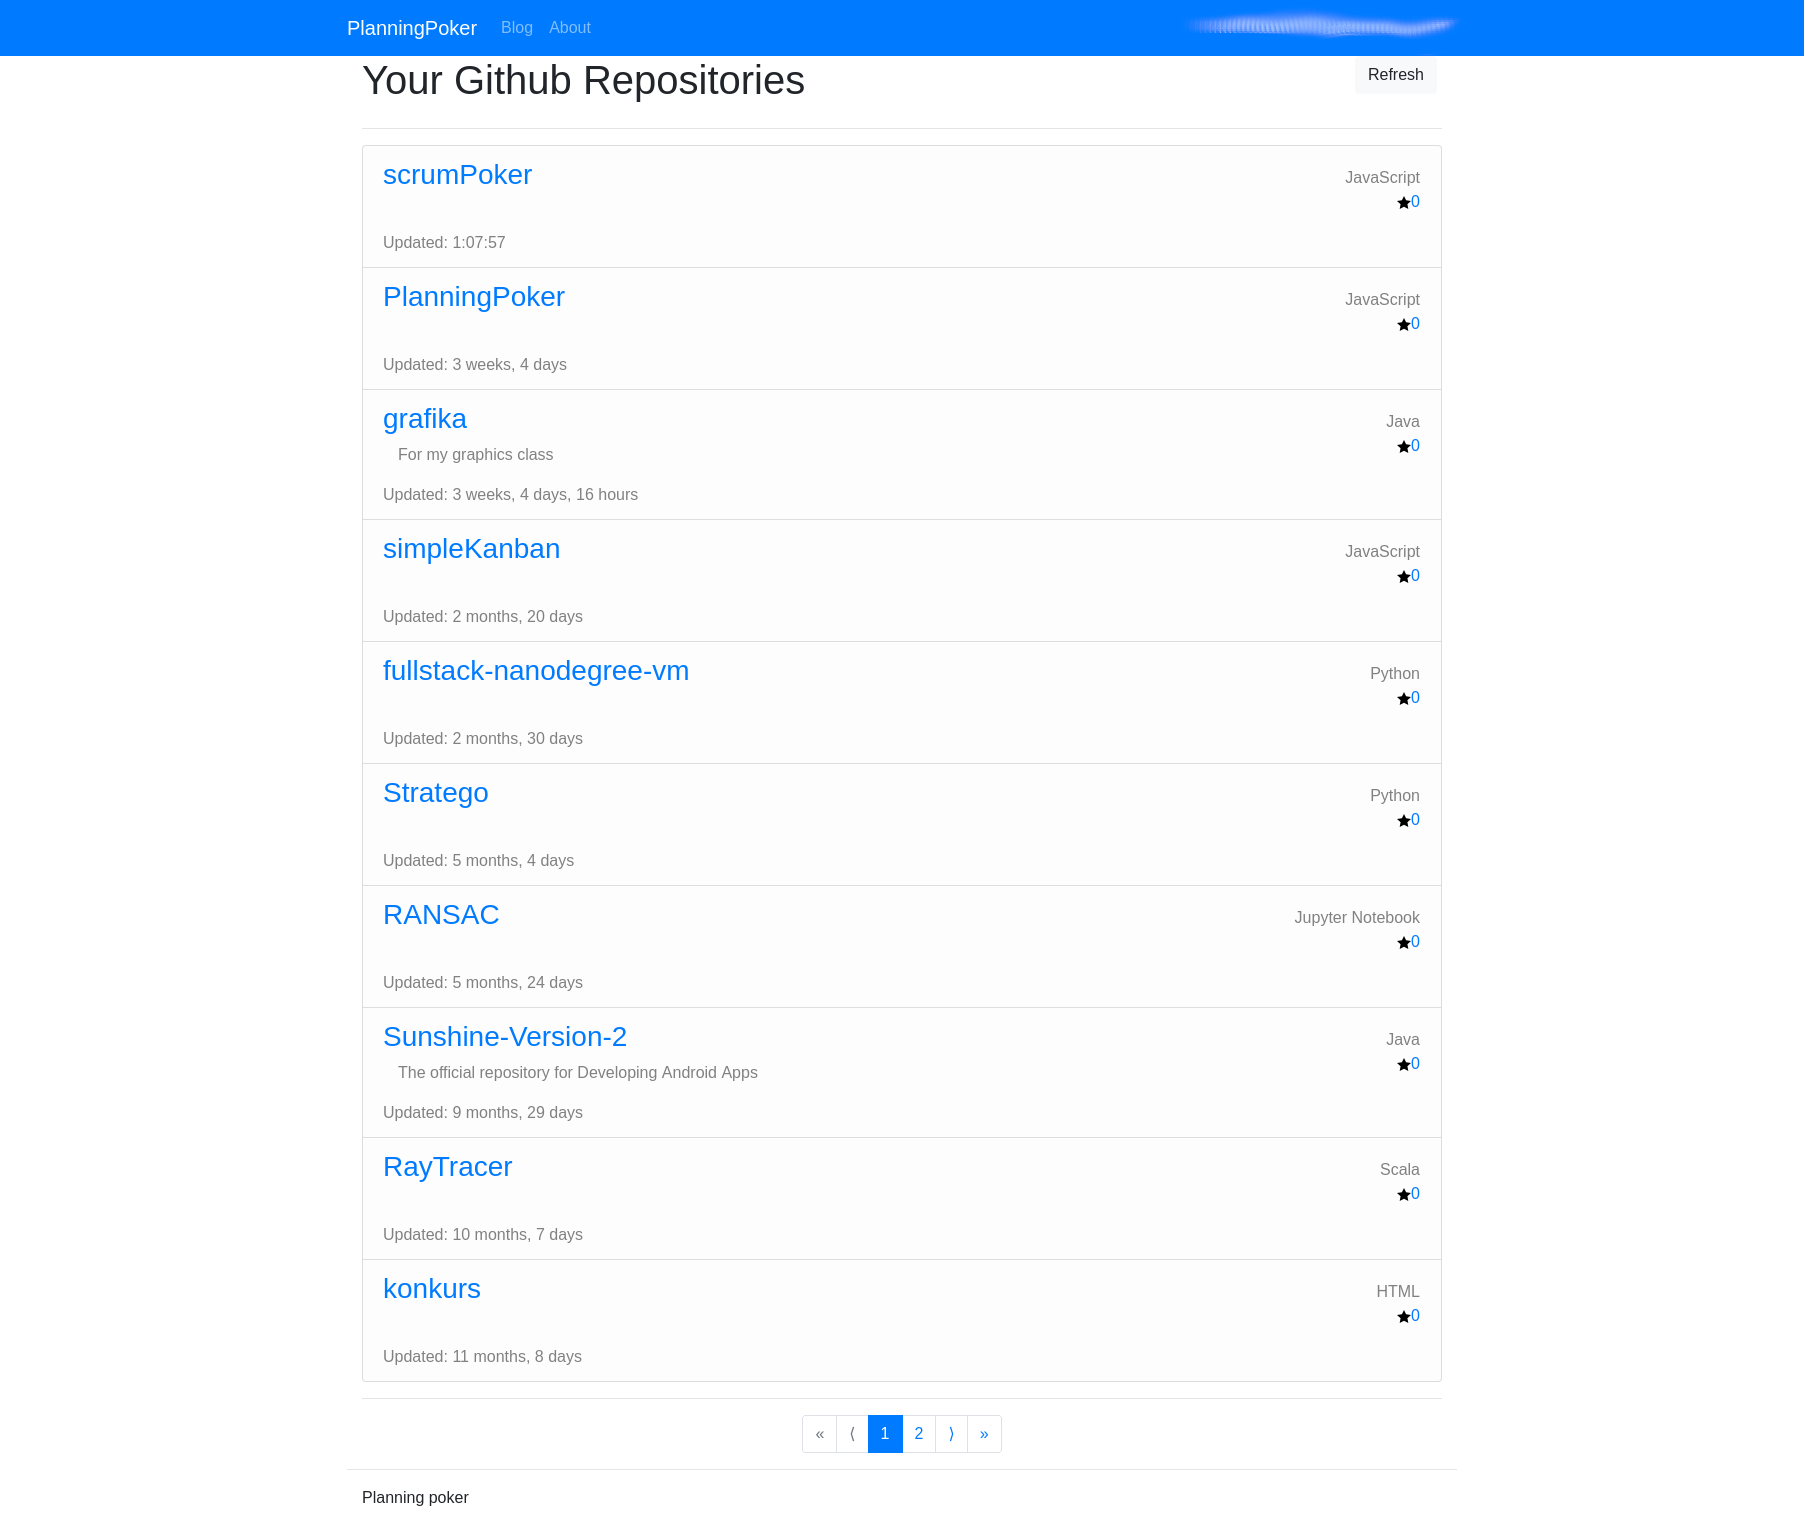
\includegraphics[width=\textwidth]{img/repositories.png}
	\caption{Ekran wyboru projektu}\label{rys:projekty}% Źródło rysunku i etykieta przez którą odwołujemy się do rysunku.
\end{figure}

Autor podczas przeglądania projektów na Github'ie zauważył, że jego użytkownicy,
wszelkie problemy czy też propozycje nowych funkcjonalności aplikacji umieszczają
w sekcji \textbf{issues} danego projektu. Stwierdził wówczas, iż aplikacja która ocenia
istniejące problemy lub proponowane cechy, które są dostępne w już sprawdzonym narzędziu
i eksportuje oceny do Github'a w postaci etykiet będzie dobrym pomysłem.


\subsection{Ekran wyboru projektu}

Aby utworzyć grę, najpierw należy wybrać projekt, którego gra będzie dotyczyła.
W aplikacji projektami są repozytoria (rysunek~\ref{rys:projekty}).

\begin{figure}[h]
	\centering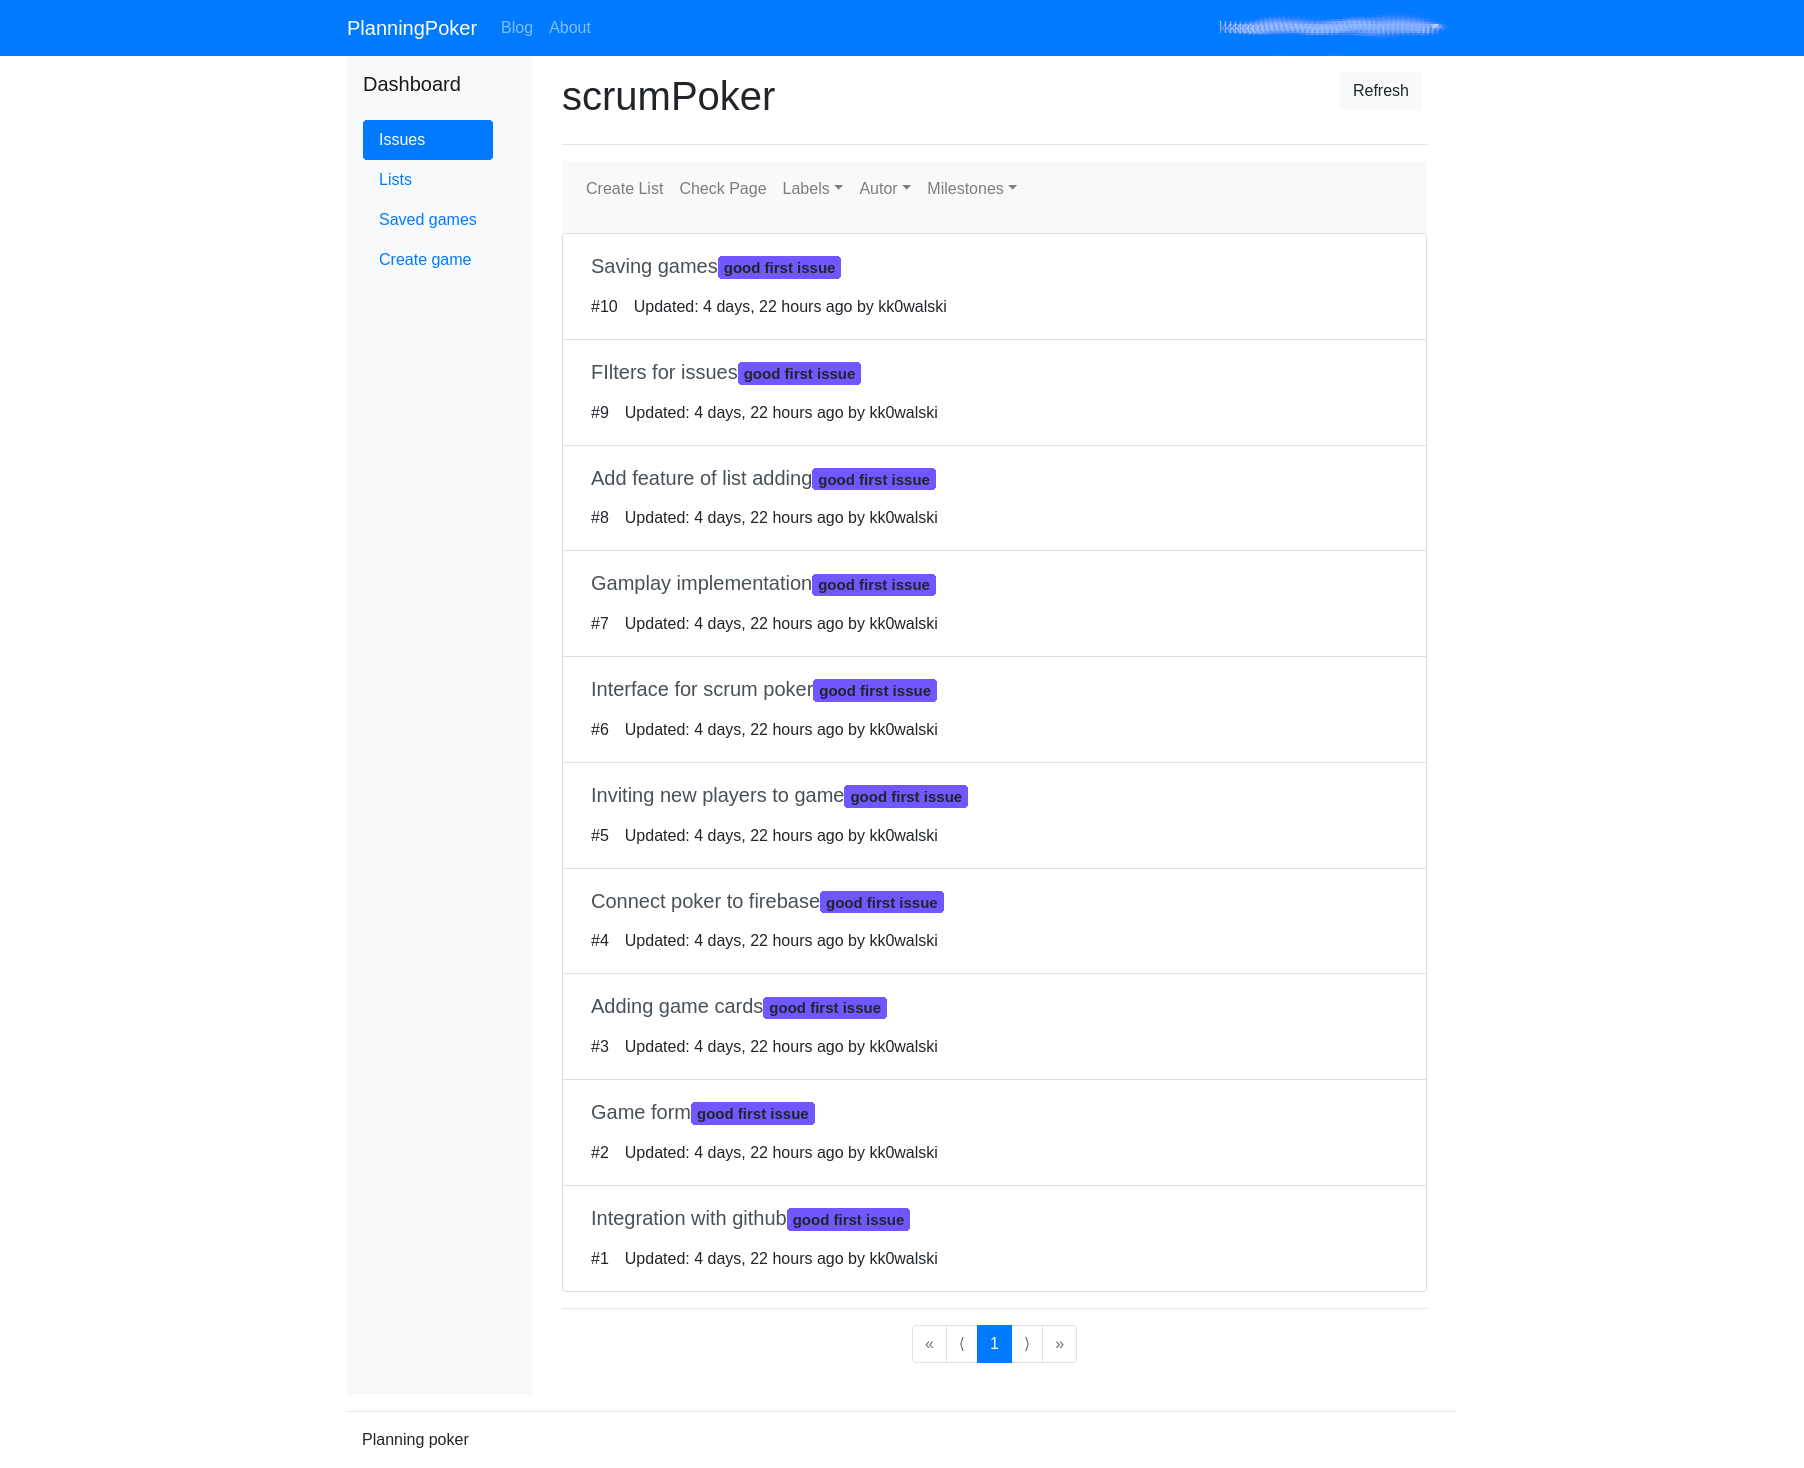
\includegraphics[width=\textwidth]{img/Issues.png}
	\caption{Ekran wyboru backlogu}\label{rys:issues}% Źródło rysunku i etykieta przez którą odwołujemy się do rysunku.
\end{figure}


\subsection{Ekran wyboru backlogu}

Aby rozgrywka miała sens, konieczne jest posiadanie backlogu zadań,
które zespół powinien wyestymować podczas danej sesji planingowej.
Odpowiednią listę zadań Tworzy się ją w panelu ustawień projektu (rysunek~\ref{rys:issues}),
w sekcji \textbf{Issues}.

Dzięki odpowiednim ustawieniom filtrów można odnaleźć elementy po etykietach,
autorze czy po kamieniach milowych.

Aby stworzyć listę, należy wybrać odpowiednie zagadnienia, klikając lewy przycisk myszy,
czy też zaznaczając stronę za pomocą przycisku \textbf{Check page}.

Po wybraniu odpowiednich elementów i naciśnięciu przycisku \textbf{Create List}
pokazywane jest okno potwierdzenia,
które pokazuje wybrane elementy oraz pole do wpisania nazwy listy.

\begin{figure}[h]
	\centering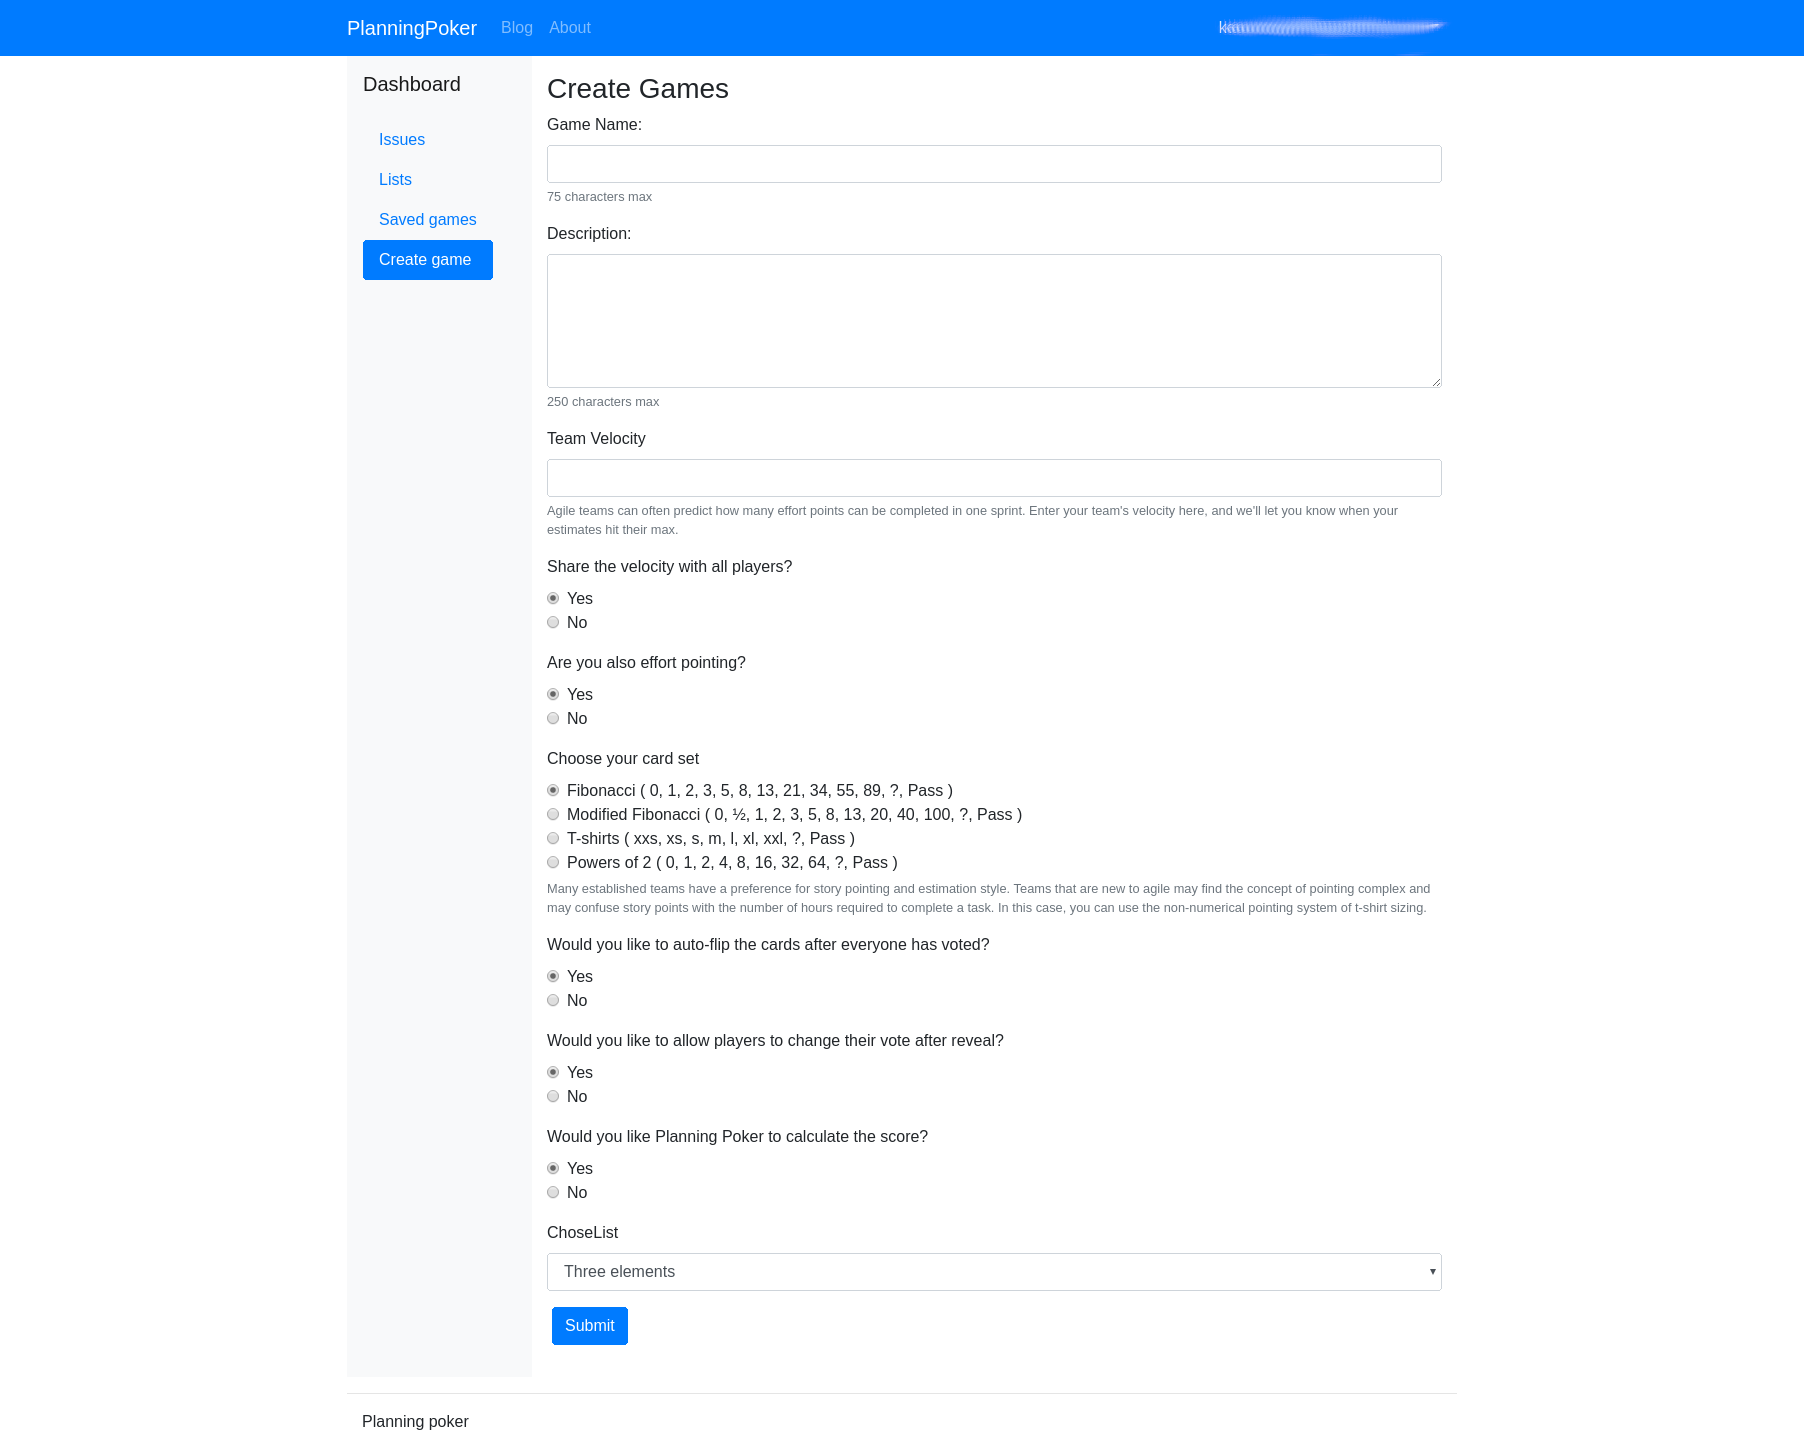
\includegraphics[width=0.8\textwidth]{img/formularz.png}
	\caption{Formularz tworzenia gry}\label{rys:form}% Źródło rysunku i etykieta przez którą odwołujemy się do rysunku.
\end{figure}

Po potwierdzeniu wyboru oraz wpisaniu nazwy listy, jest tworzona lista, zawierająca
identyfikatory wybranych historyjek (czyli \textit{issues} w projekcie Github).

Jak zostało już wcześniej wspomniane, niezbędnym elementem gry jest backlog.
Tym backlogiem dla każdej gry będzie lista, którą właściciel tworzy spośród wspomnianych historyjek.
Ta lista będzie później dostępna w formularzu tworzenia gry,
dzięki czemu będzie można ją wybrać przy jej tworzeniu.


\subsection{Ekran ustawień gry}

W trakcie tworzenia gry możemy skorzystać z ekranu ustawień gry (rysunek~\ref{rys:form})
aby określić jej nazwę i opis ale także parametry, które będą miały wpływ na grę.
Oczywiście, będziemy mogli wybrać skalę estymacji gry, ale także podać prędkość (ang.\ velocity)
naszego zespołu, zdecydować czy inni gracze będą tą prędkość widzieć.
Możemy także zdecydować czy twórca gry również będzie mógł głosować.

Inną ważną kwestią jest to, czy karty powinny być odkrywane, kiedy każdy zagłosował
oraz czy pozwolić graczom zmienić swoją ocenę po pokazaniu wszystkich kart.

Aplikacja może również obliczać wynik punktowy historyjki po zakończonym głosowaniu automatycznie,
robi to za pomocą średniej ważonej, która później jest zamieniana na najbliższą jej ocenę w skali estymacji.

Na końcu oczywiście należy wybrać backlog w postaci odpowiedniej listy, tu należy zaznaczyć,
że jeżeli w projekcie nie będzie stworzonej żadnej listy, to nie będzie można stworzyć gry.

Pewne ustawienia gry można zmienić także już po jej utworzeniu.

\section{Rozgrywka}

Do rozgrywki Planning Pokera oczywiście potrzebni są gracze.
Aby rozgrywka była możliwa dla więcej niż jednego gracza, konieczna jest komunikacja z serwerem.
Wszelkie akcje podczas gry są synchronizowane za pomocą Firebase,
a dzięki odpowiednim słuchaczom aplikacja reaguje na wszelkie zmiany w stanie gry.

Gracz jest dodawany do gry poprzez udostępnianie innym użytkownikom odnośnika do gry
w postaci jej adresu URL\@.
Jeżeli gracz wejdzie do gry, zostanie poproszony o podanie nazwy,
dzięki której będzie można go odróżnić od innych graczy.
Gracze są dodawani do bazy danych dzięki funkcji usługi Firebase nazwanej anonimowe logowanie.
Gracze w grze mogą tylko i wyłącznie głosować,
natomiast właściciel gry wybiera historyjkę do głosowania, to znaczy że to on narzuca tempo gry.
Panel gry pokazuje rysunek~\ref{rys:gra}.

\begin{figure}[h]
	\centering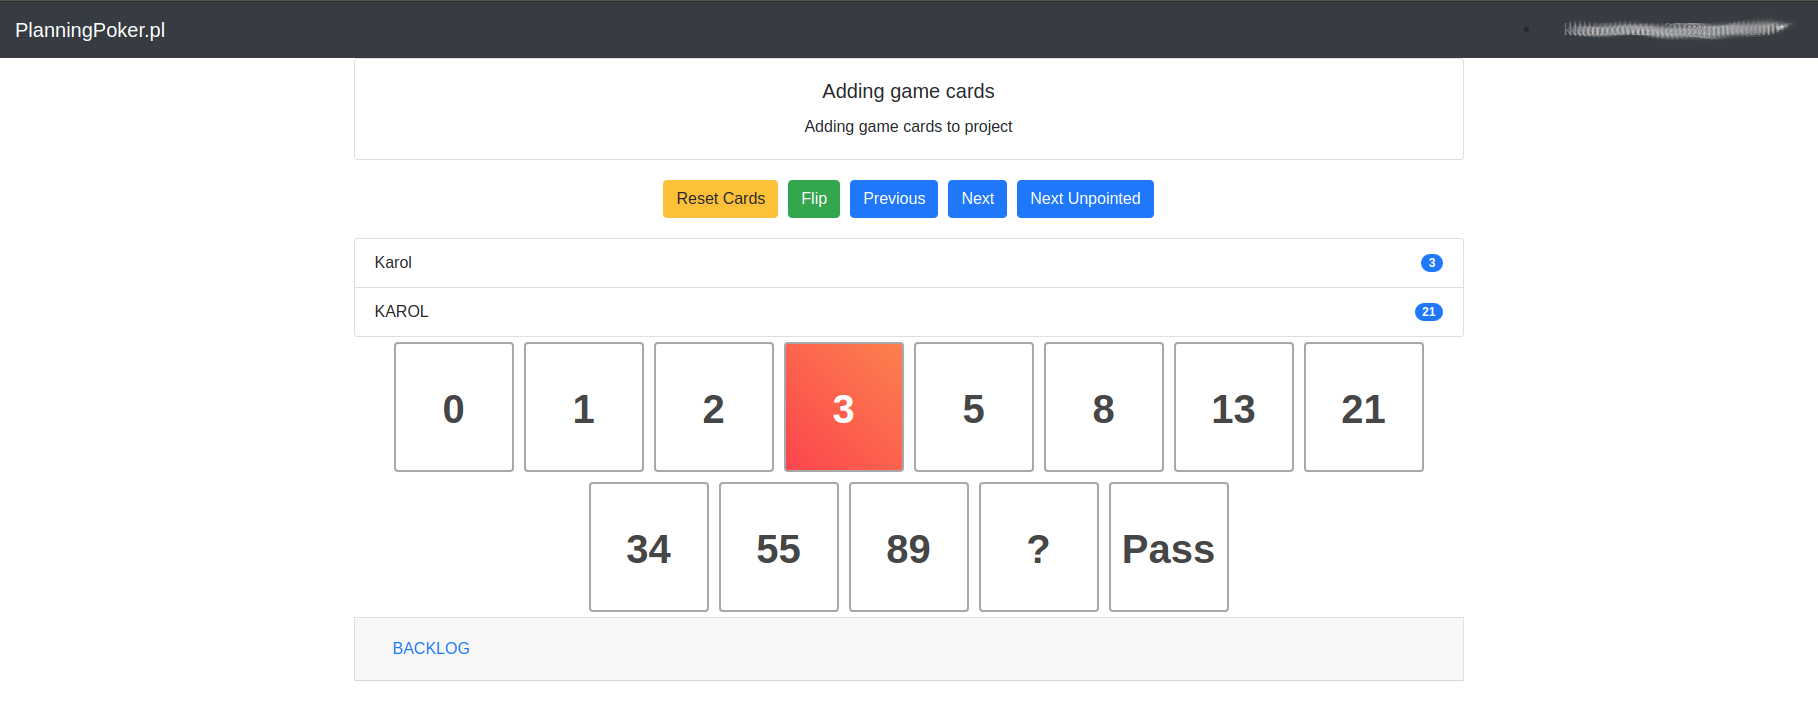
\includegraphics[width=\textwidth]{img/gra.png}
	\caption{Panel gry}\label{rys:gra}% Źródło rysunku i etykieta przez którą odwołujemy się do rysunku.
\end{figure}

\section{Komunikacja słowna}

Istotnym elementem każdego Planning Pokera jest komunikacja między graczami,
autor jednak stwierdził,
iż na rynku istnieją już odpowiednie aplikacje do komunikacji,
a firmy produkujące oprogramowanie mają preferowane komunikatory, których używają
również w innych sytuacjach niż proces planowania sprintu.
A więc przed każdą rozgrywką autor poleca wybrać odpowiedni komunikator do komunikacji w trakcie gry.


\section{Wynik implementacji}

Nie wszystkie zaplanowane elementy znajdują się w aplikacji,
jednak najważniejsze funkcjonalności zostały zaimplementowane:

 \begin{itemize}
	\item Logowanie przez Github'a
	\item Pobieranie Issues z Github'a
	\item Tworzenie list, które będą backlog'iem w grze
	\item Tworzenie gier
	\item Rozgrywka
	\item Eksport wyników gier do Github'a
	\item Możliwość usunięcia gry
	\item Możliwość zmiany ustawień gry
	\item Możliwość zapraszania użytkowników do gry
\end{itemize}

Funkcje których nie udało się zaimplementować to:

\begin{itemize}
	\item Pełna synchronizacja z Github'em
	\item Edycja historyjek wraz z synchronizacją zmian z Github'em
	\item Możliwość usuwania użytkownika z gry
\end{itemize}

\section{Podsumowanie}

Dzięki użyciu odpowiednich technologii udało się stworzyć w pełni funkcjonalną aplikację,
umożliwiającą zespołom zdalnym przeprowadzenie sesji planningowej nad dobrze
zdefioniowanym backlogiem zadań.
Nie znaczy to jednak, że jej stworzenie było proste.
Autorowi zajęło trochę czasu zanim wybrał odpowiednie technologie do projektu.
Można powiedzieć że niniejsza praca była świetną okazją do poznania
wielu nowych narzędzi do tworzenia aplikacji internetowych wykorzystujących
komunikację w czasie rzeczywistym.
